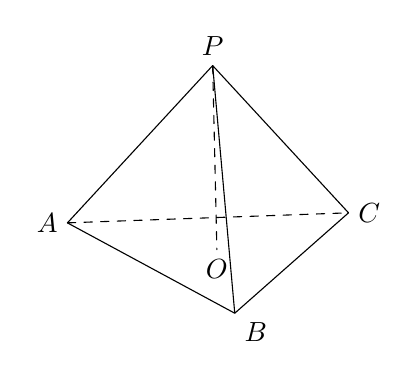
\begin{tikzpicture}[line cap=round,line join=round,scale=0.85]
  \coordinate (A) at (-2.15,0.20);
  \coordinate (B) at (0.35,-1.15);
  \coordinate (C) at (2.05,0.35);
  \coordinate (O) at (0.083,-0.20);
  \coordinate (P) at (0.02,2.55);

  % Hidden far edge and altitude in the source drawing.
  \draw[dashed] (A)--(C) (P)--(O);
  % Visible base edges and lateral edges.
  \draw (A)--(B)--(C) (P)--(A) (P)--(B) (P)--(C);

  \node[left] at (A) {$A$};
  \node[below right] at (B) {$B$};
  \node[right] at (C) {$C$};
  \node[below] at (O) {$O$};
  \node[above] at (P) {$P$};
\end{tikzpicture}
